\begin{SingleSpace}
\chapter{Non-Linear Tests of a Linear Theory of Tidally Locked Atmospheres}
\vspace{0.5cm}
\chapterprecishere{``One might as well approximate the derivatives well instead of badly''\par\raggedleft--- \textup{John P. Boyd}, Chebyshev and Fourier Spectral Methods}
\end{SingleSpace}
\vspace{0.5cm}



%0 -- LEAD-IN PARAGRAPHS

%START ELEMENT

In this chapter, I test the mechanism for the circulation of tidally locked planetary atmospheres predicted in the previous chapter. I use a single-layer non-linear shallow-water model, and a 3D General Circulation Model (GCM) to simulate the atmosphere, and compare the results to the linear theory.

%FRAMING TEXT

The linear theory simplified the system of a tidally locked planetary atmosphere greatly, and these tests will investigate whether these assumptions were accurate, and test how well the theory predicts the equilibrium circulation.

%SIGNPOSTS

I will introduce the models used, and show basic tests of whether the mechanism predicted by the linear model is actually at work. I will test the spin-up and equilibrium states of the non-linear models, and compare the results to the scaling relations predicted by the linear model.

%SUMMARISE CONCLUSIONS

This chapter will show that the linear model is a good approximation to the results of the non-linear simulations. The wave-mean flow interaction in the linear theory also applies to the non-linear simulations, suggesting that this is at work on real tidally locked planetary atmospheres as well.



%SECTION 1 -- NONLINEAR TESTS
\section{Non-Linear Tests of Linear Shallow-Water Theory}

% RUN:
% 3 no-jet tests with different h forcing
% 1 default spin-up with jet forcing
% Scaling tests

The linear model in Chapter \ref{ch:wave-mean-flow} made X main simplifications:

\begin{enumerate}
  \item The perturbations to the atmosphere are small enough to be approximately linear.
  \item The atmospheric response is (on average) stationary, and any transient behaviour does not affect the mean circulation.
  \item The atmosphere and the variations in it are small enough in the vertical to be approximated by a shallow model.
  \item The day-night forcing is approximated by a relaxation to a constant radiative equilibrium height field.
\end{enumerate}

This section discusses tests of the single-layer linear theory in Chapter \ref{ch:wave-mean-flow} using a single-layer non-linear model, which removes the first two assumptions.


%SUBSECTION -- MODEL
\subsection*{Non-Linear Shallow-Water Model}

I used the Geophysical Fluid Dynamics Laboratory Flexible Modelling System (FMS) Spectral Dynamical Core (GFDL-SDC) for non-linear shallow-water simulations. Appendix \ref{ap:gfdl-sdc} describes the model setup.

%SUBSECTION -- LINEARITY
\subsection*{Testing Linearity}

The linear model in Chapter \ref{ch:wave-mean-flow} is based on a forced linear shallow-water system as discussed in \citet{matsuno1966quasi}. Figure \ref{fig:linear-matsuno-response} shows the response to a forcing $Q(x,y) = \sin(x) e^{-y^{2}/2}$ in this linear system.

\begin{figure}
  \centering
    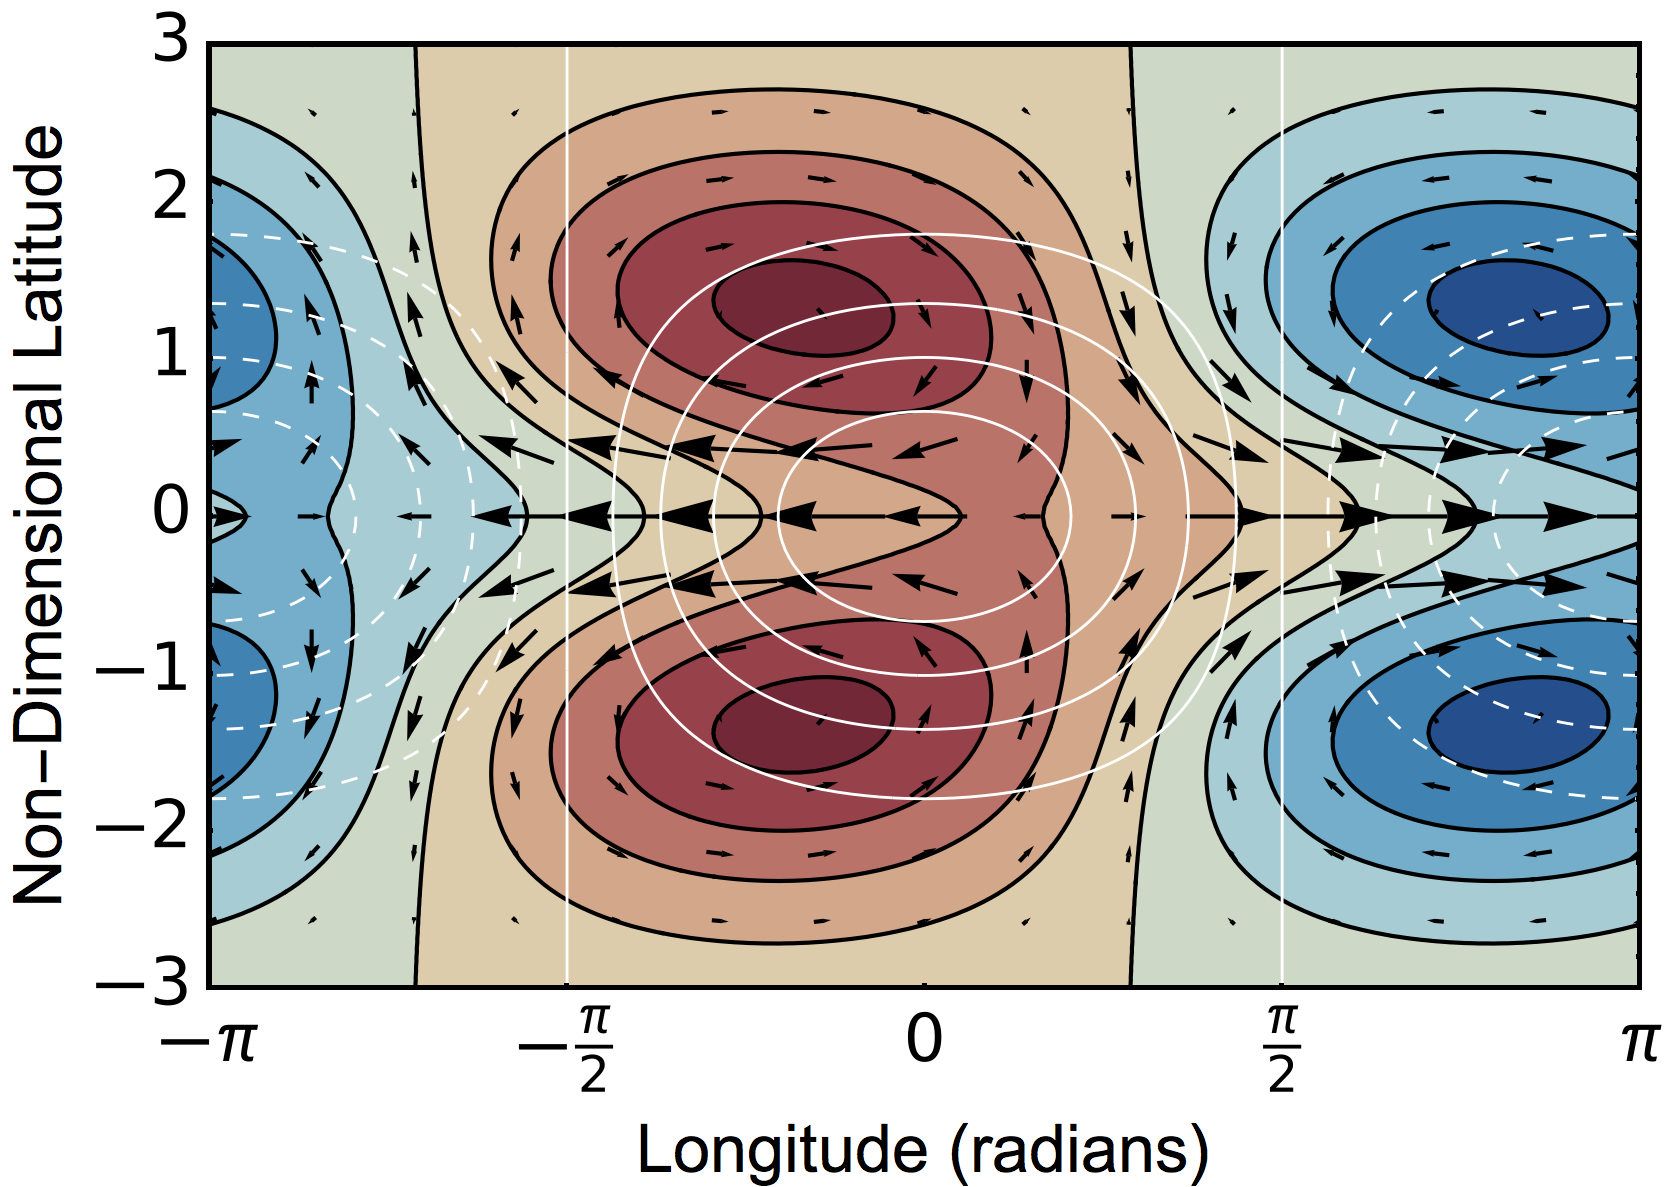
\includegraphics[width=0.5\textwidth]{figures/nonlinear-circulation/motivate-showman.png}
    \caption{The linear response.}
    \label{fig:linear-matsuno-response}
\end{figure}

The linear model assumes that the perturbations in the shallow-water system (representing perturbations in a real three-dimensional atmosphere) are small enough that the linear terms dominate the shallow-water equations. I ran simulations in the non-linear shallow-water model to test whether they matched the linear model at appropriate forcing strength.

The non-linear shallow-water equations are:

The linear solution in spherical coordinates in Figure X in Chapter X has $\alpha_{rad} = \alpha_{dyn} = 0.2$, $G = 1$ and $\Delta h / H = 0.5$. To match this in the non-linear model, I set $\alpha_{rad} = \alpha_{dyn} = 0.2$, $\Delta h = 5\ \textrm{km}$, and $ H = 10\ \textrm{km}$. To set $G=1$, I set $R=R_{Earth}$ and $g=10$, then tuned the rotation rate to $\Omega = 4.964\times10^{-5}=0.6807\Omega_{Earth}$.

Figure \ref{fig:nonlinear-matsuno-control} shows the equilibrated height and velocity fields for the non-linear model with these parameters, and zero imposed background flow. The non-linear model matches the linear model in Figure X well, with a similar pattern and perturbation size. There is a small day-night asymmetry in the non-linear mode which is not present in the linear model.

The plots in Figure \ref{fig:nonlinear-matsuno} show the non-linear response with a smaller height perturbation $\Delta h = 1\ \textrm{km}$, and a larger height perturbation $\Delta h = 20\ \textrm{km}$. Figure \ref{fig:nonlinear-matsuno-1e3} with the smaller perturbation has a smaller day-night asymmetry than Figure X.b, which is expected as the smaller perturbation should produce a more linear response. Figure \ref{fig:nonlinear-matsuno-1e4} with the larger perturbation has a larger day-night asymmetry than Figure \ref{fig:nonlinear-matsuno-control}, which is expected as the larger perturbation should produce a less linear response. The pattern is also more different from the linear pattern, showing that the linear approximation is less appropriate at the higher forcing amplitude.

This is all as expected, and shows that the forcing amplitudes used in the linear solutions in Chapter X ($\Delta h / (H \tau_{rad} \sim 0.1$) and the GCM simulations in Chapter X ($\Delta T / (T \sim 0.1$) are in a regime that is well represented by the linear approximation.


\begin{figure}
  \centering
  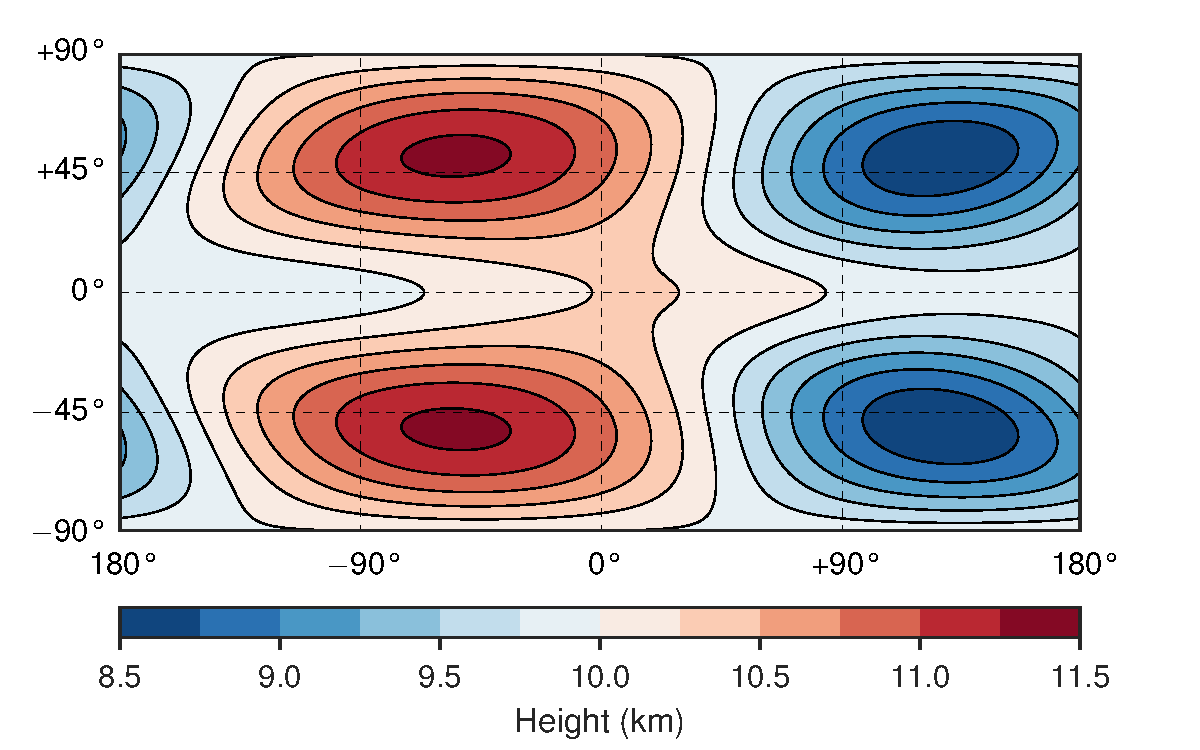
\includegraphics[width=0.5\textwidth]{figures/nonlinear-circulation/nonlin-matsuno-5e3.pdf}
  \caption{5e3.}
  \label{fig:nonlinear-matsuno-control}
\end{figure}


\begin{figure}
  \begin{subfigure}[b]{0.5\textwidth}
    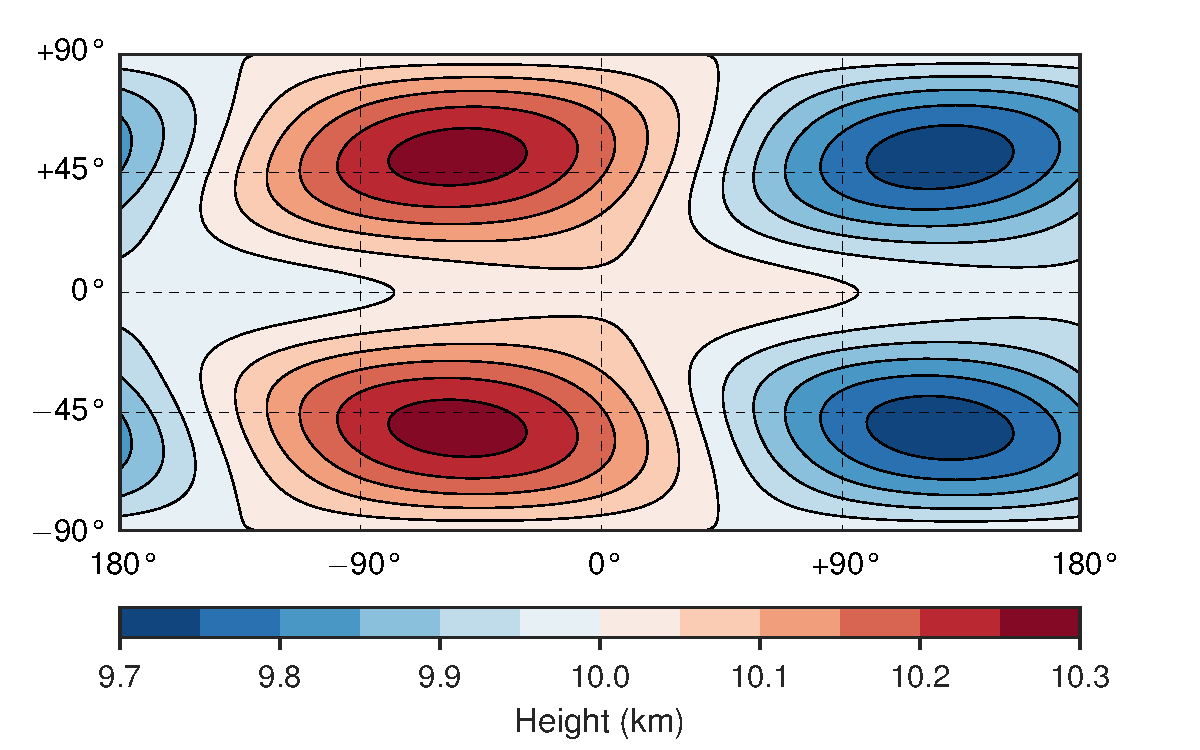
\includegraphics[width=1.0\textwidth]{figures/nonlinear-circulation/nonlin-matsuno-1e3.pdf}
    \caption{1e3.}
    \label{fig:nonlinear-matsuno-1e3}
  \end{subfigure}
  %
  \begin{subfigure}[b]{0.5\textwidth}
    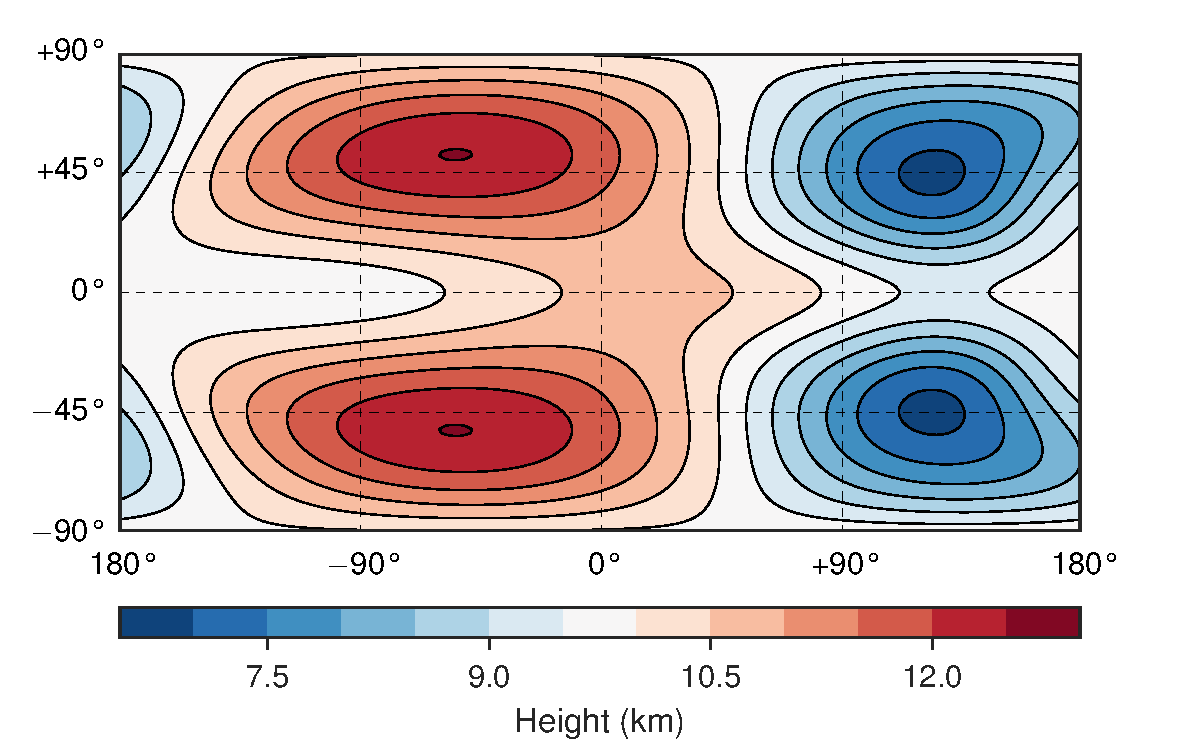
\includegraphics[width=1.0\textwidth]{figures/nonlinear-circulation/nonlin-matsuno-1e4.pdf}
    \caption{1e4.}
    \label{fig:nonlinear-matsuno-1e4}
  \end{subfigure}
  \caption{Nonlinear.}
  \label{fig:nonlinear-matsuno}
\end{figure}

It is possible that the background flow that is imposed in the linear solutions and emerges in the GCM simulations affects the size of the perturbations and moves the system out of the linear regime. I ran the same non-linear shallow-water simulations as Figure X, but imposed the same jet as in the linear solutions to test if the linear and non-linear solutions still matched.

The simulations had the same parameters as in Figure \ref{fig:nonlinear-matsuno-control}. The linear model in spherical geometry in Chapter X has a jet with a non-dimensional velocity of $0.5 \cos \phi \exp(-(\phi/\phi_{0})^{2})$, with a jet width $\phi_{0} = \pi/3$. The non-linear system in Figure \ref{fig:nonlinear-matsuno-control} has a velocity scale of $R \Omega$, so I relaxed the non-linear simulations on a timescale $\tau_{dyn} = 1 / \alpha_{dyn}$ to a background flow profile $R \Omega \cos \phi \exp(-(\phi/\phi_{0})^{2})$. Figure \ref{fig:matsuno-jet-control} shows the equilibrated response.

The non-linear response has much less shift at higher latitudes, and a much narrower zonal height field. The zonal flow profile is much narrower than the imposed profile. Figure X shows that subtracting the background flow that is imposed leaves a large retrograde flow in the midlatitudes, as forms in the non-linear Matsuno case. Figure X shows the response and the mean zonal velocity of the case which is not relaxed towards a background flow (the same test as Figure \ref{fig:nonlinear-matsuno-control}). This case has westward flow in the midlatitudes, as predicted by Figure X in Chapter X. This mechanism causes the reduced eastward flow in the midlatitudes in the case with a jet in Figure X.


This is responsible for the main difference between the linear and non-linear model. In fact, the acceleration calculated in the linear model does predict this westward midlatitude flow, but it was ignored in Chapter X to match the GCM results.

This highlights a difference between the GCM and the shallow-water models. The shallow-water models always predict a westward acceleration in the mid-latitudes, but this is rarely seen in the GCM. In Chapter X I suggest that eastward acceleration from Rossby wave breaking is responsible for the midlatitude eastward flow in the GCM.

These simulations have shown that the linear model is an appropriate approximation for the atmosphere of a tidally locked planet, but that it does not correctly predict the acceleration away from the equator.

\begin{figure}
  \centering
  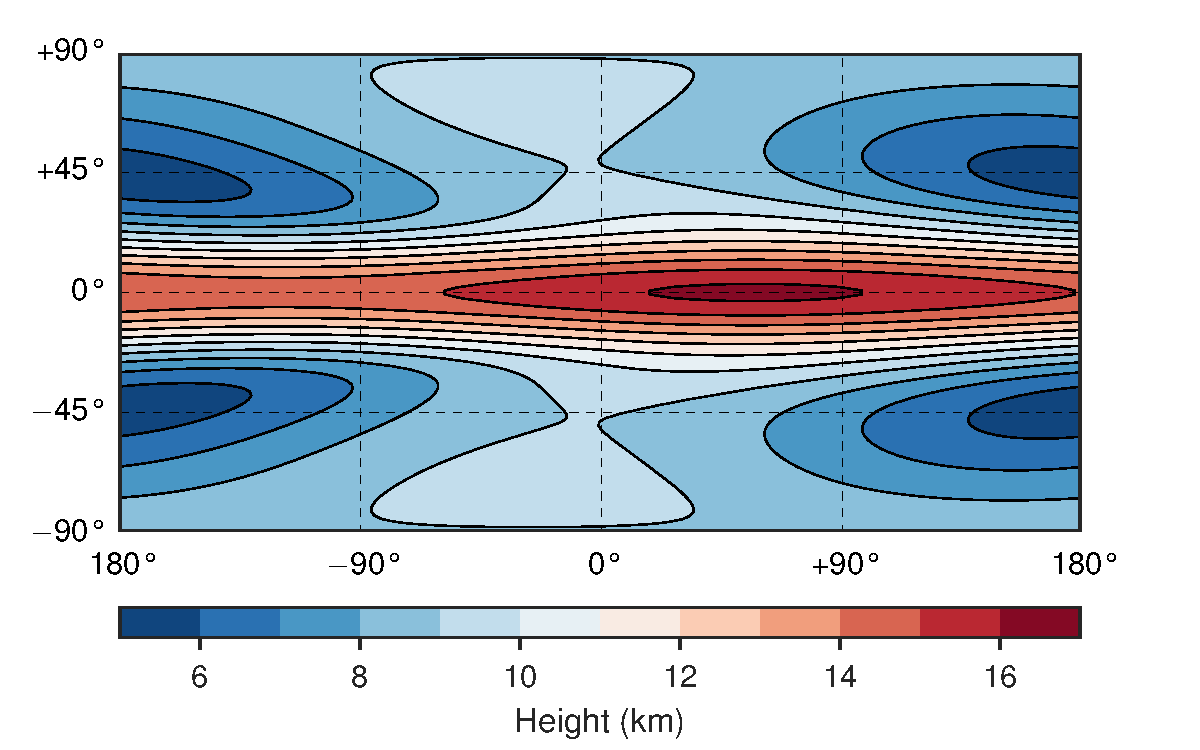
\includegraphics[width=0.5\textwidth]{figures/nonlinear-circulation/matsuno-jet-control.pdf}
  \caption{Matsuno jet control.}
  \label{fig:matsuno-jet-control}
\end{figure}

\begin{figure}
  \begin{subfigure}[b]{0.33\textwidth}
    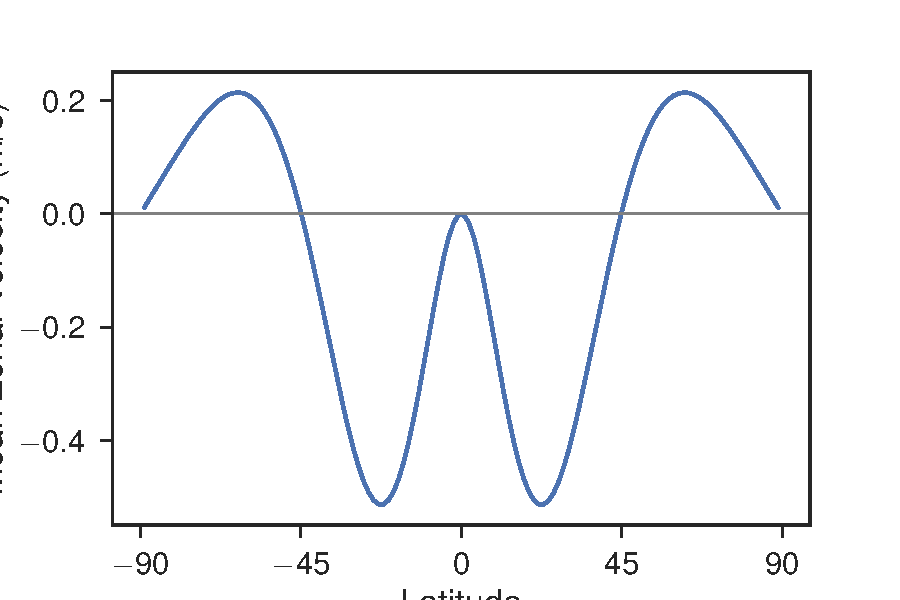
\includegraphics[width=1.0\textwidth]{figures/nonlinear-circulation/m-control_mean-u.pdf}
    \caption{m-control_mean-u.}
    \label{fig:m-control_mean-u}
  \end{subfigure}
  %
  \begin{subfigure}[b]{0.33\textwidth}
    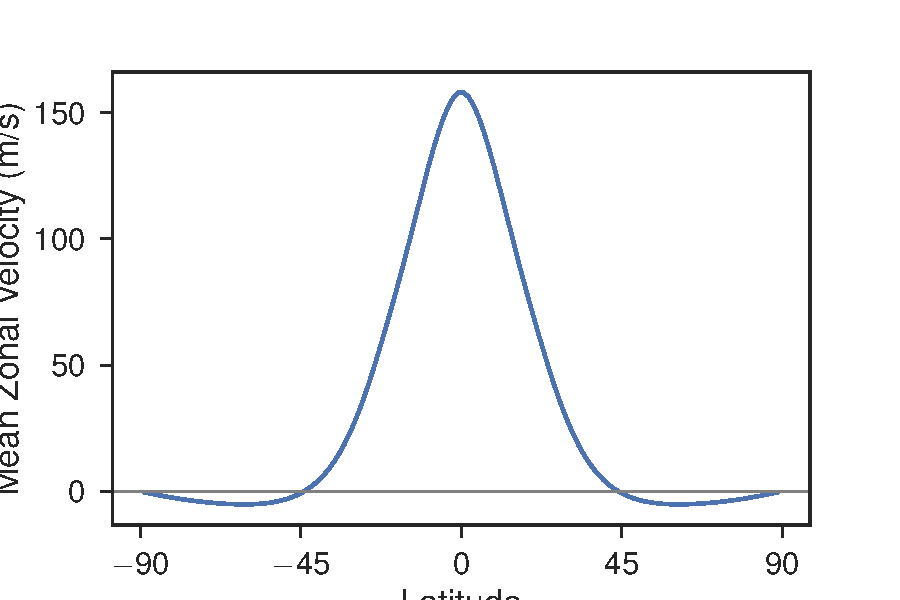
\includegraphics[width=1.0\textwidth]{figures/nonlinear-circulation/m-jet-control_mean-u.pdf}
    \caption{m-jet-control_mean-u.}
    \label{fig:m-jet-control_mean-u}
  \end{subfigure}
  %
  \begin{subfigure}[b]{0.33\textwidth}
    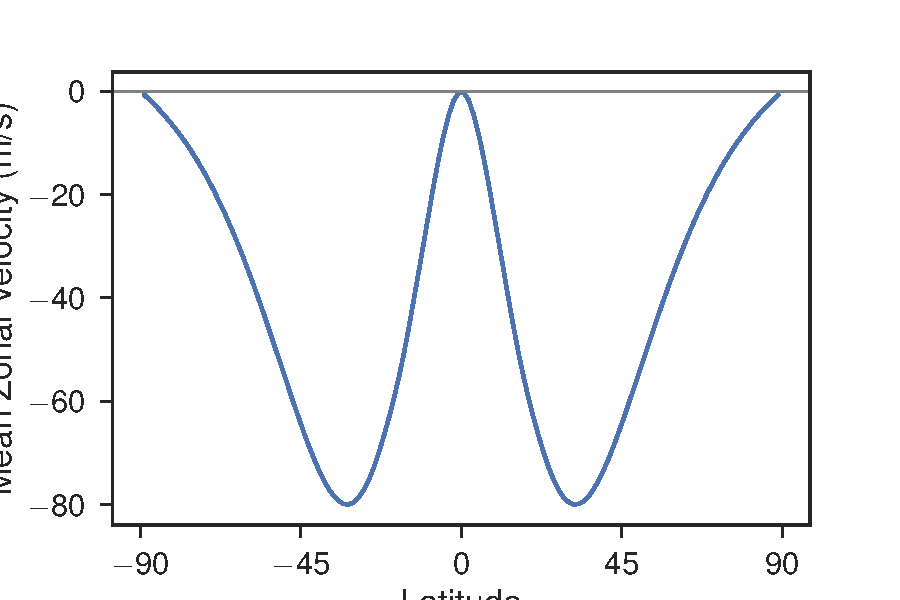
\includegraphics[width=1.0\textwidth]{figures/nonlinear-circulation/m-jet-control_mean-u-minus-U.pdf}
    \caption{m-jet-control_mean-u-minus-U.}
    \label{fig:m-jet-control_mean-u-minus-U}
  \end{subfigure}
  \caption{Nonlinear.}
  \label{fig:m-jet-control_mean-u_figure}
\end{figure}



%SUBSECTION -- EQUILIBRIUM
\subsection*{Testing Equilibrium State}

Chapter X discusses the jet acceleration.

The time-stepped model reaches an equilibrium state after about X days. The transient response from the impulse generated by turning on the forcing dissipates, and a steady state is reached.

Show wave components, hot-spot, and wind directions.

Figure X shows the equilibrium state for the model with forcing X and rotation rate X. Figure X shows the eddy state, showing how the waves have shifted.


%SUBSECTION -- SPIN-UP
\subsection*{Testing Jet Spin-up}

I ran tests to show how the atmosphere reaches this state.

Figure X shows the eddy state over time of the previous test.

Figure X shows the Rossby and Kelvin components over time of the previous test.

Spin-up of height field, eddy height field, and Rossby and Kelvin components.


%SUBSECTION --  SCALING TESTS
\subsection*{Scaling Relation Tests}

Test effect of rotation rate, forcing, jet speed.

Figure X shows the equilibrium state for the model with the same forcing X and different rotation rates X.

Figure X shows the equilibrium state for the model with different forcing X.

Figure X shows the equilibrium state for the model with different jet speed X.

%SECTION 2 -- GCM TESTS
\section{GCM Tests of Shallow-Water Theory}

I used the GCM Exo-FMS, based on the Geophysical Fluid Dynamics Laboratory Flexible Modelling System (GFDL-FMS). Chapter \ref{ch:sim-exofms} and Appendix \ref{ap:exo-fms} describe this model.

%SUBSECTION -- EQUILIBRIUM
\subsection*{Testing Equilibrium State}

Show wave components, hot-spot, and wind directions.

%SUBSECTION -- SPIN-UP
\subsection*{Testing Jet Spin-up}

Spin-up of height field, eddy height field, and Rossby and Kelvin components.

%SUBSECTION --  SCALING TESTS
\subsection*{Scaling Relation Tests}

Test effect of rotation rate, forcing, jet speed.


%SECTION CONCLUSIONS




%CONCLUSIONS

%RESTATE SECTION CONCLUSIONS

%OPEN OUT CONCLUSIONS


% \bibliographystyle{unsrtnat}
% \bibliography{../references.bib}
